\documentclass{article}
    \usepackage{amssymb}
    \usepackage[utf8]{inputenc}
    \usepackage[russian]{babel}
    \usepackage[left=2cm,right=2cm,
        top=2cm,bottom=2cm,bindingoffset=0cm]{geometry}
    \usepackage{hyperref}
    \hypersetup{
        colorlinks=true,
        linkcolor=blue,
        filecolor=magenta,      
        urlcolor=cyan,
    }
  \usepackage{graphicx}
  \usepackage{booktabs}
  \usepackage{hyperref}
  \graphicspath{{pictures/}}
  \DeclareGraphicsExtensions{.pdf,.png,.jpg}
\usepackage{subcaption}
%\captionsetup{compatibility=false}

\begin{document}
\begin{center}{\hugeОтчет по дипломной работе за неделю\\}\end{center}
Дата: 8.4.2021\\
Научные руководители: Герасимов С.В., Мещеряков А.В.\\
Студент: Немешаева Алиса\\
Курс: 4\\

\renewcommand{\labelitemi}{$\blacksquare$}
\renewcommand\labelitemii{$\square$}
\begin{enumerate}
    \item Перестроены гистограммы ~\ref{Fig:Hist} для оценки случайно найденных скоплений в 
        каталоге. Новые графики были построены следующим образом:\\
        \begin{enumerate}
            \item Для каждого детектированного скопления в <<красную>> выборку добавляются все 
                скопления из ground-truth каталога, которые попали а радиус $400''$ от выбранного 
                детектированного объекта (для прошлой версии графика записывалось только ближайшее
                скопление).\\
            \item Аналогично в <<синюю>> выборку добавляются \textbf{все} скопления, найденные в 
                радиусе $[400'',\; 1500'']$.\\
            \item Такой способ позволяет более точно оценить количество случайно обнаруженных 
                скоплений.\\
        \end{enumerate}
    \item Построена новая модель. В обучающую выборку для этой модели добавлялись все скопления из 
        каталогов MCXC, Abell, ACT, RedMaPPer, что были найдены в самом удачном детектированном 
        каталоге (pz\_all\_found\_34). Результаты полученного каталога на валидационной выборке в
        таблице.\\
        %\ref{Tab:Recall}{}.\\
    \item Построены случайно сгенерированные каталоги ~\ref{Fig:Rnd_map} с разным количеством 
        объектов. Эти каталоги --- ещё один способ оценить количество случайно найденных объектов 
        с полученном каталоге. Также проведено сопоставление с детектированным каталогом и 
        построен график соответствия количеству найденных объектов в зависимости от радиуса 
        ~\ref{Fig:Rnd}.\\
\end{enumerate}




\begin{figure}[h]
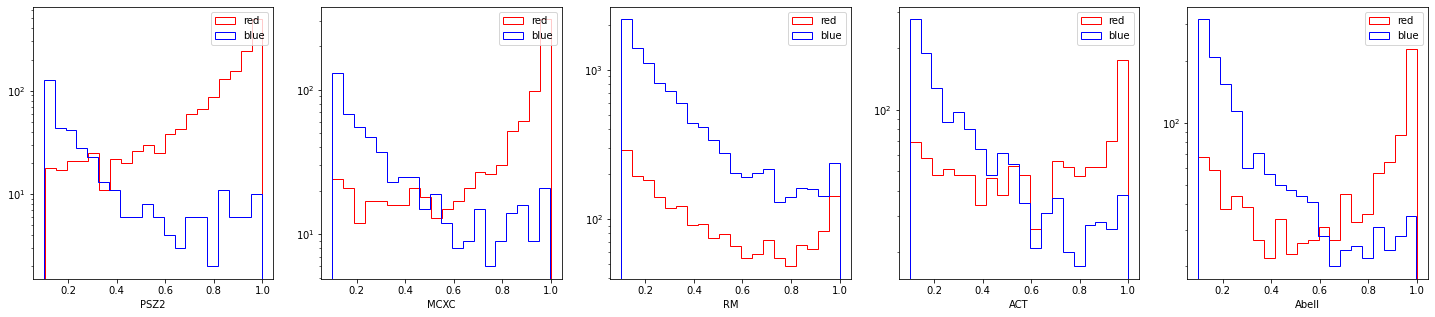
\includegraphics[width=\linewidth]{hist}
\caption{Распределение всех найденных объектов и ошибочно найденных объектов}
\label{Fig:Hist}
\end{figure}

\begin{table}[h]
\begin{tabular}{lrrrrrrr}
\toprule
{} &     PSZ2 &      MCXC &        RM &       ACT &     Abell &    fp &   all \\
\midrule
pz14                        &  0.93125 &  0.439759 &  0.043817 &  0.220930 &  0.213429 &   872 &  1181 \\
pz\_rot28                    &  0.95000 &  0.463855 &  0.048685 &  0.225914 &  0.227818 &  1194 &  1531 \\
pz\_act\_rot\_drop0.1\_ep9      &  0.91875 &  0.427711 &  0.037326 &  0.186047 &  0.196643 &   542 &   815 \\
pz\_act\_jan\_rot\_drop0.1\_ep6  &  0.93750 &  0.409639 &  0.038624 &  0.179402 &  0.215827 &   625 &   903 \\
pz\_act\_feb\_rot\_drop0.3\_ep14 &  0.92500 &  0.427711 &  0.055826 &  0.235880 &  0.249400 &  1576 &  1938 \\
pz\_act\_q\_0.1\_0.9\_14         &  0.94375 &  0.469880 &  0.048685 &  0.230897 &  0.225420 &  1201 &  1536 \\
pz\_act\_found2\_22            &  0.93750 &  0.463855 &  0.053879 &  0.249169 &  0.235012 &  1145 &  1504 \\
pz\_all\_found34              &  0.95000 &  0.481928 &  0.058423 &  0.244186 &  0.249400 &  1268 &  1644 \\
pz\_all\_found2\_34            &  0.94375 &  0.493976 &  0.059072 &  0.244186 &  0.247002 &  1445 &  1821 \\
pz\_found0.8\_20              &  0.93750 &  0.487952 &  0.056800 &  0.225914 &  0.235012 &  1230 &  1587 \\
pz\_found0\_28                &  0.94375 &  0.469880 &  0.052256 &  0.235880 &  0.247002 &  1318 &  1670 \\
\bottomrule
\end{tabular}
\label{Tab:Recall}
\caption{Таблица recall для различных построенных моделей на валидационной выборке.}
\end{table}

\begin{figure}[h]
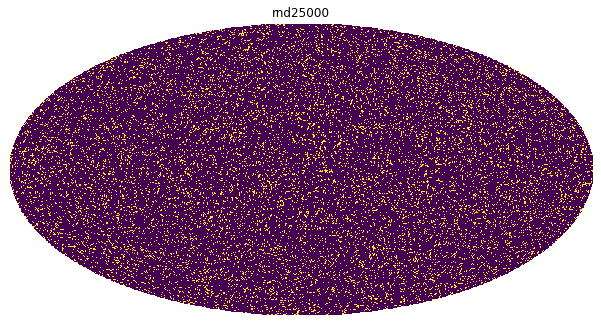
\includegraphics[width=0.7\linewidth]{rnd_map}
\caption{Карта случайно сгенерированных объектов (25000 объектов).}
\label{Fig:Rnd_map}
\end{figure}

\begin{figure}[h]
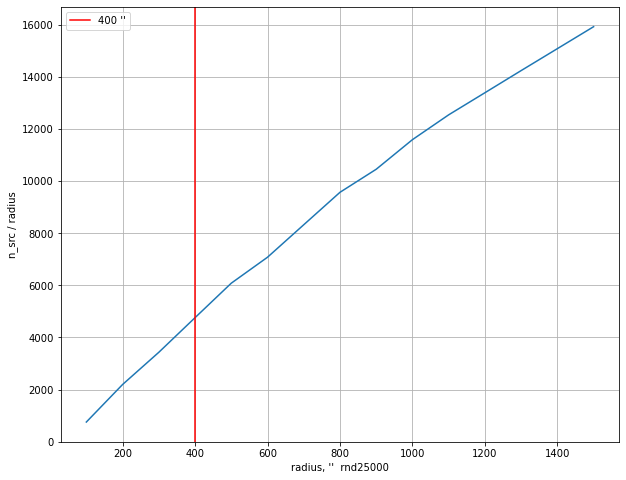
\includegraphics[width=0.6\linewidth]{rnd}
\caption{Количество случайно найденных объектов в зависимости от радиуса сопоставления.}
\label{Fig:Rnd}
\end{figure}

Отчет согласован с научным руководителем.\\
Общее количество строк кода за эту неделю: 299\\
\href{https://github.com/rt2122/data-segmentation-2}{Репозиторий}\\ 
\end{document}
